\documentclass{article}
\usepackage{fullpage}
\usepackage{amsmath}
\usepackage{braket}
\usepackage[sort&compress,numbers,super]{natbib}
\usepackage{achemso}
\usepackage{graphicx}
\usepackage{array}
\usepackage{tikz}
\usepackage{circuitikz}
\usepackage{url}
\usepackage{epigraph}
\begin{document}
\title{Efficient Parametrization and Solution of the Electronic Wavefunction on a Quantum Processor: A Review}
\author{Harper Grimsley}

\maketitle
\setlength \epigraphwidth {\linewidth}
\epigraph{\centering With four parameters I can fit an elephant, and with five I can make him wiggle his trunk.}{John Von Neumann}
\tableofcontents
\section{Classical Chemistry Methods}
\subsection{Hartree-Fock}
\begin{paragraph}{}
The Hartree-Fock (HF) approximation is a self-consistent field (SCF) approximation to the electronic structure of a molecule, based on approximately solving equation \ref{bsl} for the various orbitals, $\{\chi\}$, via linear variation. \cite{szabo} (This equation is essentially a restatement of the time-dependent Schr{\"o}dinger equation in the syntax of Slater determinants.)
\begin{equation} \label{bsl}
E_0 =\sum_{i}\Braket{\chi_i|\hat{H}|\chi_i}+\sum_{i<j}\Braket{\chi_i\chi_j|\chi_i\chi_j}-\Braket{\chi_i\chi_j|\chi_j\chi_i}
\end{equation}
While variational and size-consistent, HF fails to capture dynamical correlation, and therefore overestimates chemical energies. \cite{szabo}\cite{jensen} In spite of its lack of chemical accuracy, The SCF method is formally only O$\left(N^4\right)$ where N is the number of molecular orbitals. (This comes from the number of 2-electron integrals.) \cite{szabo}\cite{jensen} Furthermore, it provides a single-configuration wavefunction which can function as a reference for more powerful iterative methods. \cite{szabo}  An alternative view of the HF state is that it exactly solves the Hamiltonian in \ref{hfham}.
\begin{equation} \label{hfham}
\hat{H_0}=\sum_i\hat{f}\left(i\right)
\end{equation}
The term $\hat{f}\left(i\right)$ is the Fock operator associated with the position and spin of electron i, defined in equation \ref{fockop}. \cite{szabo}
\begin{equation} \label{fockop}
\hat{f}\left(i\right)=\hat{h}\left(i\right)+\sum_{j}\hat{\mathcal{J}}_j\left(i\right)+\hat{\mathcal{K}}_j\left(i\right)
\end{equation}
In equation \ref{fockop}, $\hat{h}$ accounts for nuclear attraction of electron i to the nucleus, $\hat{\mathcal{J}}$ accounts for the mean Coulombic interaction between electrons i and j, and $\hat{\mathcal{K}}$ accounts for the mean ``exchange" interaction between electrons i and j. \cite{szabo} Because electron j is assumed to be fixed and described by its average contributions to each term, this is a single-electron operator. \cite{szabo}  This definition of the HF state is helpful for describing perturbation theory. \cite{szabo} 
\end{paragraph}



\subsection{Configuration Interaction}
\begin{paragraph}{}
While HF theory considers the single best electronic configuration of a system, configuration interaction (CI) theory allows for linear combinations of all configurations, seeking the ideal solution of the form in equation \ref{ci}. \cite{szabo}
\begin{equation}\label{ci}
c_{0}\ket{\Psi^{\left(0\right)}}+\sum_{i,a}c_{ij}\ket{\Psi_i^a}+\sum_{i,j,a,b}c_{ijab}\ket{\Psi_{ij}^{ab}}+...
\end{equation}
In full CI, every level of excitation is included to yield the exact basis set limit energy of the system. \cite{szabo} Unfortunately, there are O$\left(N!\right)$ coefficients in equation \ref{ci}, making full CI intractable ``for all but the very smallest systems." \cite{szabo,jensen} Alternatively, it is possible to truncate at a fixed number of excitations to reduce computational complexity. \cite{jensen} Only including single excitations does nothing by Brillouin's theorem, so at least double excitations need to be included. \cite{szabo}  CI with single and double excitations (CISD) is O$\left(N^6\right)$; the addition of triple excitations (CISDT) gives O$\left(N^8\right)$, the addition of quadruple excitations (CISDTQ) gives O$\left(N^{10}\right)$, and so on. \cite{jensen}  This scaling originates from the number of determinants in each excitation scheme. \cite{jensen} All CI schemes are constructed to be variational; however, only full CI is size-consistent, making truncated CI progressively worse for increasingly large molecules. \cite{atkins} For this reason, truncated CI is considered inappropriate for large systems, with methods like perturbation theory and coupled cluster used in its place. \cite{szabo,atkins} Therefore, no form of CI is applicable to most systems of interest.  
\end{paragraph}



\subsection{Perturbation Theory}
\begin{paragraph}{}
One approach to improve on a reference state is to consider the exact Hamiltonian $\hat{H}$ as the Hartree-Fock Hamiltonian, $\hat{H}_0$, with a small perturbation $\hat{\mathcal{V}}$. \cite{szabo}
\begin{equation} \label{perturb}
\hat{H}=\hat{H}_0+\hat{\mathcal{V}}
\end{equation}
Similarly, we can expand the exact wavefunction $\ket{\Psi}$ as a sum of corrections to the HF wavefunction, $\ket{\Psi^{\left(0\right)}}$, as shown in equation \ref{wfnper}, and expand the ground-state energy E as a sum of corrections to the HF energy, $E^{\left(0\right)}$, as shown in equation \ref{eper}. \cite{szabo}\cite{atkins}
\begin{equation} \label{wfnper}
\ket{\Psi}=\ket{\Psi^{\left(0\right)}}+\lambda\ket{\Psi^{\left(0\right)}}+\lambda^2\ket{\Psi^{\left(0\right)}}+...
\end{equation}
\begin{equation}\label{eper}
E = E^{\left(0\right)}+\lambda E^{\left(1\right)}+\lambda^2 E^{\left(2\right)}+...
\end{equation}
Breaking up these corrections by the order of expansion parameter $\lambda$, which can hereafter be ignored, gives an arbitrarily large number of equations, as given below. \cite{atkins}  (Note that the perturbative correction to the Hamiltonian is of first order.)
\begin{align*}
\hat{H}_0\ket{\Psi^{\left(0\right)}}&=E_0\ket{\Psi^{\left(0\right)}}\\
\hat{H}_0\ket{\Psi^{\left(0\right)}}+\hat{\mathcal{V}}\ket{\Psi^{\left(0\right)}}&=E_0\ket{\Psi^{\left(1\right)}}+E_1\ket{\Psi^{\left(0\right)}}\\
\hat{H}_0\ket{\Psi^{\left(2\right)}}+\hat{\mathcal{V}}\ket{\Psi^{\left(1\right)}}&=E_0\ket{\Psi^{\left(2\right)}}+E_1\ket{\Psi^{\left(1\right)}}+E_2\ket{\Psi^{\left(0\right)}}\\
&...
\end{align*}
Sequentially solving these equations gives M{\o}ller-Plesset (MP) perturbation theory, a non-iterative, size-consistent method for finding any arbitrary order of correction to the Hartree-Fock wavefunction and energy. \cite{atkins}  Perturbation theory can be done to any order n, using MPn.  MP1, however, does nothing by Brillouin's theorem. \cite{jensen}  The most common form, MP2 is O$\left(N^5\right)$, due to the four-index orbital transformation to molecular orbitals from atomic orbitals. \cite{jensen} MP3 is O$\left(N^6\right)$, MP4 is O$\left(N^7\right)$, and so on due to increasing numbers of energy terms to evaluate. \cite{jensen}\cite{diner}\cite{pulay} Furthermore, the MP procedure is ``not particularly accurate", and is non-variational. \cite{pulay}\cite{pulay2}
\end{paragraph}

\subsection{Coupled Cluster}
\begin{paragraph}{}
Coupled cluster (CC) theory, like MP theory, sacrifices the variational property for size consistency. \cite{atkins}  CC theory is generally truncated to single and double excitations (CCSD), single, double, and triple excitations (CCSDT), and so on. \cite{crawford}  The coupled cluster ansatz for a given truncation level is given in equation \ref{cc}. \cite{crawford}
\begin{equation}\label{cc}
e^{\sum\limits_{ia}t_i^a a_a^\dagger a_i+\frac{1}{4}\sum\limits_{ijab}t_{ij}^{ab} a_a^\dagger a_b^\dagger a_j a_i+...}\ket{\Psi^{\left(0\right)}}\equiv e^{\hat{\mathcal{T}}_1+\hat{\mathcal{T}_2}+...}\ket{\Psi^{\left(0\right)}}\equiv e^{\hat{\mathcal{T}}}
\end{equation}
This form of the wavefunction allows one to separate the wavefunction of two isolated systems into a single product wavefunction, which gives the method its size consistency. \cite{szabo}\cite{crawford} We can non-variationally solve for the t-amplitudes in equation \ref{cc} by similarity transfoming the Hamiltonian using the cluster operator, then considering the projections by the reference state and by each excited state, giving equations \ref{crawf} and \ref{crawf2}. \cite{crawford}
\begin{equation}\label{crawf}
\Braket{\Psi^{\left(0\right)}|e^{-\hat{\mathcal{T}}}\hat{H}e^{\hat{\mathcal{T}}}|\Psi^{\left(0\right)}}=E
\end{equation}
\begin{equation}\label{crawf2}
\Braket{\Psi_{ij...}^{ab...}|e^{-\hat{\mathcal{T}}}\hat{H}e^{\hat{\mathcal{T}}}|\Psi^{\left(0\right)}}=0
\end{equation}
The Baker-Campbell-Hausdorff (BCH) expansion enables the similarity-transformed Hamiltonian to be evaluated as a truncating sum of nested commutators. \cite{crawford} The exact details of solving the t-amplitudes from equations \ref{crawf} and \ref{crawf2} are beyond the scope of this work.  It suffices to note that CCSD scales as O$(N^6)$, CCSDT scales as O$(N^8)$, and so on. \cite{jensen}  
\end{paragraph}


\subsection{Unitary Coupled Cluster}
\begin{paragraph}{}
In ordinary coupled cluster theory, the BCH expansion gives a finite number of terms to evaluate; the tradeoff is that the cluster operator is not generally unitary, meaning coupled cluster is not variational.  \cite{crawford} An alternative approach is to replace $\hat{\mathcal{T}}$ with $\hat{\mathcal{T}}-\hat{\mathcal{T}}^\dagger$. \cite{hoffman}  The parametrization of this new operator $\mathcal{T'}$ is as shown in equation \ref{ucc}. \cite{crawford}\cite{hoffman}
\begin{equation}\label{ucc}
\hat{\mathcal{T'}}=\sum_{ia}t'_{ia}\left(a_a^\dagger a_i-a_i^\dagger a_a\right)+\sum_{ijab}t'_{ijab}\left(a_a^\dagger a_b^\dagger a_j a_i-a_i^\dagger a_j^\dagger a_b a_a \right)+...
\end{equation}
This generator is, by construction, anti-Hermitian, thus making $e^{\hat{\mathcal{T}}}$ unitary. \cite{hoffman,gallier}  The unitary character of 
$$e^{\hat{\mathcal{T}}}=e^{-\hat{\mathcal{T}}^\dagger}$$
makes equations \ref{crawf} and \ref{crawf2} variational when $\hat{\mathcal{T}}$ is replaced by $\hat{\mathcal{T'}}$ \cite{crawford} Unfortunately, the BCH expansion no longer truncates in unitary coupled cluster, demanding a finite number of terms be included. \cite{crawford,hoffman,evangelista,bartlett} Unitary coupled cluster theory is not considered practical for real systems due to the exponentially increasing cost of solving equations \ref{crawf} and \ref{crawf2}. \cite{evangelista,joonho,bartlett} There are other variational coupled cluster schemes with similar limitations, but we restrict our discussion to Hoffman's formulation. \cite{hoffman,crawford,evangelista}  Of the classical chemistry methods described, only unitary coupled cluster methods can be truncated to a fixed level of excitation while preserving the variational principle and maintaining size consistency.  Its only downside is classical intractability; this serves as sufficient motivation to explore the application of quantum computers to quantum chemistry.
\end{paragraph}


\section{Quantum Information Background}
\subsection{Qubits}
\begin{paragraph}{}
In classical computer science, all information is compressed to bits, binary units of information with value of either 0 or 1. \cite{nielsen}  The quantum analogue of a bit is a qubit, which is assigned any unit vector in $\mathbf{C}^2$, as shown in equation \ref{qubit}. \cite{nielsen}
\begin{equation}\label{qubit}
\ket{\Psi} = \alpha\ket{0}+\beta\ket{1}\equiv \begin{pmatrix}\alpha\\ \beta \end{pmatrix}
\end{equation}
Furthermore, a qubit obeys all of the postulates of quantum mechanics, making it intuitively useful for simulating quantum mechanical problems. \cite{nielsen}\cite{feynman} A system can exist with more than one qubit; for example, the state in equation \ref{pure} is a pure 2-qubit state, while the state in equation \ref{ent} is an entangled 2-qubit state.
\begin{equation}\label{pure}
\ket{\Psi}=\ket{00}
\end{equation}
\begin{equation}\label{ent}
\ket{\Psi}=\frac{1}{\sqrt{2}}(\ket{00}+\ket{11})
\end{equation}
Note that both states maintain the unit normalization condition.  A pure 2-qubit state is one in which the outcomes are uncorrelated or \textit{unentangled}.  Entanglement describes how much the state of one qubit affects the other; for example, the qubit in equation \ref{ent} is \textit{maximally entangled} because one qubit cannot be measured without collapsing the state of the other to match.
\end{paragraph}
\begin{paragraph}{}
Measuring the state of a qubit is more complicated than measuring the state of a bit.  Consider the arbitrary qubit in equation \ref{qubit}; quantum mechanics tells us that if we measure in the computational basis, we can get only outcomes $\ket{0}$ or $\ket{1}$ with probabilities given by equations \ref{p0} and \ref{p1}.
\begin{equation}\label{p0}
P\left(\ket{0}\right)=\left|\braket{0|\Psi}\right|^2=|\alpha|^2
\end{equation}
\begin{equation}\label{p1}
P\left(\ket{1}\right)=\left|\braket{1|\Psi}\right|^2=|\beta|^2
\end{equation}
The physics literature tends to refer to this technique as projective measurement, and define the measurement operator M for state $\ket{\phi}$ by equation \ref{measurement}. \cite{nielsen}
\begin{equation}\label{measurement}
M = \ket{\phi}\bra{\phi}
\end{equation}
This convention can be helpful when one is interested in the state of a system post-measurement, since it enacts the state collapse.  (The measurement operator does not renormalize the state; this must be done separately.)  The projective measurement equations \ref{p0} and \ref{p1} in this notation are given by equations \ref{p02} and \ref{p12} respectively. \cite{nielsen}
\begin{equation}\label{p02}
P(\ket{0})=\braket{\Psi|0}\braket{0|0}\braket{0|\Psi}=|\alpha|^2
\end{equation}
\begin{equation}\label{p12}
P(\ket{1})=\braket{\Psi|1}\braket{1|1}\braket{1|\Psi}=|\beta|^2
\end{equation}
In general, the probability of measuring $\ket{\Psi}$ in the state described by M is given in equation \ref{meas}. \cite{nielsen}
\begin{equation}\label{meas}
P = \bra{\Psi}M^\dagger M\ket{\Psi}
\end{equation}
We now consider the case of measuring an arbitrary 2-qubit state, as given in equation \ref{2q}.
\begin{equation}\label{2q}
\ket{\Psi}=\alpha\ket{00}+\beta\ket{01}+\gamma\ket{10}+\delta\ket{11}
\end{equation}
Measuring both qubits simultaneously works the same way as measuring a single qubit; the only difference is that there are four orthogonal states the two qubits can be in.  Measuring one qubit does not generally collapse the other qubit, so we need to apply the measurement operator to see what happens to the state.  Consider the case where we measure the first qubit to be in state $\ket{0}$.  Then the measurement operator is $\ket{0}_1\bra{0}_1$, and we partially collapse our state according to equation \ref{parti}.
\begin{equation}\label{parti}
\ket{0}_1\bra{0}_1\ket{\Psi}=\ket{0}_1\otimes(\alpha\braket{0|0}_1\ket{0}_2+\beta\braket{0|0}_1\ket{1}_2+\gamma\braket{1|0}_1\ket{0}_2+\delta\braket{1|0}_1\ket{0}_2)=\alpha\ket{00}+\beta\ket{01}
\end{equation}
Evauluating the probabilities of measuring $\ket{\Psi}$ to be in each basis state is performed according to equation \ref{meas}; the tensor bookkeeping works similarly to equation \ref{parti}. Finally, it is worth noting that the global phase of a qubit is computationally irrelevant; many algorithms take advantage of this fact. \cite{nielsen}
\end{paragraph}
\subsection{Quantum Gates}
\begin{paragraph}{}
Where the bits of classical computing are replaced with quantum states, the gates of classical computers are replaced with unitary linear operators, or \textit{quantum gates}. \cite{nielsen}  The first gates we consider are the Pauli operators, $\hat{X}$, $\hat{Y}$, and $\hat{Z}$. In the computational basis, these take the forms given in \ref{x}, along with the common Hadamard, phase, and $\frac{\pi}{4}$ gates. \cite{nielsen} 
\begin{align}\label{x}
\hat{X}&=\begin{pmatrix}0&1\\1&0\end{pmatrix}&\hat{Y}&=\begin{pmatrix}0&-i\\i&0\end{pmatrix}&\hat{Z}&=\begin{pmatrix}1&0\\0&-1\end{pmatrix}\\
\nonumber\\\hat{H}&=\frac{1}{\sqrt{2}}\begin{pmatrix}1&1\\1&-1\end{pmatrix}&\hat{S}&=\begin{pmatrix}1&0\\0&i\end{pmatrix}&\hat{T}&=\begin{pmatrix}1&0\\0&e^{\frac{i\pi}{4}}\end{pmatrix}\nonumber
\end{align}
We now introduce the CNOT gate, which can change the entanglement between two qubits. \cite{nielsen}  Consider two qubits, the control and the target of the CNOT.  If the control qubit is in state $\ket{0}$, nothing happens.  If it is in state $\ket{1}$, the target qubit has the X gate applied to it, which is the quantum NOT operator.  In conjunction with the single-qubit gates listed, the CNOT gate forms a universal quantum gate set; that is, any quantum circuit can be approximated to arbitrary precision with only this set.  In fact, the Pauli gates can be excluded and this will still be a universal set. \cite{nielsen}\end{paragraph}
\begin{paragraph}{}
As a final note on gates, we introduce some basic circuit diagram notation.  Each line in a circuit diagram represents a single qubit and is read left to right. Single qubit operators are represented as labeled boxes.  CNOT gates are labeled with a dot on the control qubit, connected by a line to an open circle on the target qubit.  Other controlled unitary operators instead have a labeled box on the target qubit.  Measurements in the computational basis are shown by an electrical meter.  By default, the initial state of each qubit is assumed to be $\ket{0}$.  In figure \ref{fig:circuit}, we give a simple example, a circuit which is used to prepare the maximally entangled spin singlet state given in equation \ref{psiminus}. \cite{nielsen}
\end{paragraph}\\
\begin{figure}[h]
\begin{minipage}{.5\textwidth}
\begin{center}
\includegraphics{/home/hrgrimsl/Downloads/qasm2circ-v1.4/cirq.png}\caption{Spin Singlet Preparation Gate}\label{fig:circuit}
\end{center}
\end{minipage}%
\begin{minipage}{.5\textwidth}
\begin{equation}\label{psiminus} 
{\ket{\Psi^-}=\frac{\ket{01}-\ket{10}}{\sqrt{2}}}
\end{equation}
\end{minipage}%
\end{figure}
\subsection{Contemporary Quantum Hardware}
\subsubsection{Metrics for Quantum Utility}
\begin{paragraph}{}
We now have all of the theoretical tools to begin constructing useful algorithms.  Unfortunately, we still require some experimental ones.  A variety of experimental setups are areas of active research, but several issues persist, including state preparation, gate implementation, coherence of quantum states, and measurements. \cite{nielsen}  Physicists have quantified all of these issues and use them to assess various implemenation schemes.  We introduce a few common, related quantities in table \ref{nums}. \cite{nielsen}

\begin{table}[h]
\centering
\caption{Various Numerical Metrics}\vspace{6mm}
\begin{tabular}{m{1cm}|m{9cm}}\label{nums}
Metric & Definition \\
\hline
$T_1$ &Classical relaxation time from $\ket{1}$ to $\ket{0}$\\
$T_2$ &Coherence time of arbitrary superpositions of $\ket{1}$ and $\ket{0}$\\
$\mathcal{F}$ &Fidelity of a gate implementation\\
$t_{op}$ &Time to complete a gate implementation\\
\end{tabular}
\end{table}
\noindent These metrics will be described for each of several promising quantum computing technologies, with a focus on superconducting qubits.
\subsubsection{Superconducting Qubits}
One approach to introducing controllable quantum excitation is by controlling fluxons with a magnetic field or controlling Cooper pairs with an electric field. \cite{transmons}  The electrical case is referred to as a charge qubit or Cooper pair box, diagrammed in figure \ref{charge}. \cite{transmons}\cite{wu}
\begin{figure}[h!]\caption{Cooper Pair Box}\label{charge}
\begin{center}
\begin{circuitikz}
\draw (0,0)
to[cvsource](0,2)
to[barrier](2,2)
to[C](2,0)
to[short](0,0);
\end{circuitikz}
\end{center}
\end{figure}
By convention, the elements of the circuit are, from left to right, a capacitor, a Josephson junction, and a controlled voltage source.  The purpose of this circuit is to trap variable numbers of excess Cooper electron pairs between the Josephson junction and the capacitor on a ``superconducting island." \cite{wu}  (A Josephson junction is simply an inductor sandwiched between superconducting electrodes, such that quantum tunneling is the only mechanism of current flow through the junction.) \cite{transmons} The charge gradient on the capacitor can be controlled by the voltage applied, enabling the manual control of the number of electrons on the island. \cite{transmons,wu} Because the Josepson junction is a non-linear inductor, the island can be modeled as an anharmonic oscillator, with its lowest two eigenstates as $\ket{0}$ and $\ket{1}$. \cite{transmons} The anharmonicity is important to avoid leakage into excited states. \cite{transmons}. In practice, the high charge densities of these systems have caused high sensitivity to environmental effects, motivating the addition of a charge shunt to the design; shunted charge qubits, or \textit{transmons}, are the primary tools of our experimental collaborators. \cite{transmons}  Transmons have reasonably good coherence times on the order of 100 $\mu$s, with the unusual feature of $T_2$ and $T_1$ times being roughly equal so that $T_2$ is not the only bottleneck. \cite{nielsen,transmons} 
\end{paragraph}
\begin{paragraph}{}
Single-qubit gates are fairly easy to implement on transmons, with fidelities above 99\% typical. \cite{transmons} These are typically accomplished by driving individual qubits with microwave pulses. \cite{transmons} Only some two-qubit gates have had implementation demonstrated, with only a few achieving $\mathcal{F}>.99$. \cite{transmons} Coupling schemes between qubits are more nuanced; conceptually, the simplest is the microwave driving of one qubit at the frequency of a second qubit. Other setups allow for magnetic tuning of the qubits into resonance with one another or driving some single-qubit gate times take only a few nanoseconds, while two-qubit gate times on transmons vary from a few nanoseconds to several microseconds depending on implementation. \cite{transmons} \cite{wendin}  The fastest gates are associated with normal, 2D transmons, while the longest coherence times are associated with transmons embedded in a 3D cavity. \cite{wendin}
\end{paragraph}
\subsubsection{Other Physical Qubit Realizations}
\begin{paragraph}{}
While we are primarily interested in transmons, it is worth comparing them to other experimental setups to understand the advantages of transmons.  In the table below, we give approximate figures of merit for both transmons and other common qubit systems. \cite{wendin, bruzewicz, lucas}
\begin{table}[h!]
\centering
\caption{Comparison of Various Experimental Setups}\vspace{6mm} 
\begin{tabular}{c|c|c|c|c|c|c}\label{compare}
&$T_1$ & $T_2$ & $t_{op}$ (single-qubit) & $t_{op}$ (two-qubit) & $\mathcal{F}$ (single-qubit) & $\mathcal{F}$ (two-qubit)\\
\hline
2D Transmon&$\approx$ 40 $\mu$s &$\approx$ 40 $\mu$s&10-20 ns&10-40 ns&$\approx$ .999&$>$.99\\
3D Transmon&100 $\mu$s &$>$140 $\mu$s&30-40 ns&$\approx$ 450 ns&$>$.999&.96-.98\\
Ion Trap ($\mathrm{^{43}Ca^+}$)&$\approx$ 1s  &$\approx$1s& 1-3000 $\mu$s&$\approx$ 10$\mu$s   &$>$.99 &$>$.9999 \\
...&&&&&
\end{tabular}
\end{table}
\end{paragraph}
\begin{paragraph}{}
In reality, trapped ions represent an extremely diverse class of qubit; however, it suffices for our discussion to note that they have longer coherence times than transmons, but longer gate times.  
\end{paragraph}
\section{Quantum Algorithms for Quantum Chemistry}
\begin{paragraph}{}
We have, until now, ignored the mathematical issue of translating spin-orbitals to qubits.  This problem has several existing solutions, including the Jordan-Wigner, Bravyi-Kitaev, and parity mappings.  We offer an overview of Jordan-Wigner in appendix \ref{jw}.  Our usage of the other mappings is limited, and they are less chemically intuitive, despite in certain cases being more resource-efficient.
\end{paragraph}
\subsection{Phase Estimation Algorithm}
\begin{paragraph}{}
The phase estimation algorithm, PEA, was developed as a general way to quickly compute the spectra of large Hermitian matrices; the value of such an algorithm was quickly recognized by physicists and chemists. \cite{lloyd, alan} One possible circuit for PEA is given in figure \ref{pea}. \cite{alan, lloyd}
\begin{figure}[h!]\caption{Phase Estimation Algorithm Circuit}\label{pea}
\begin{center}
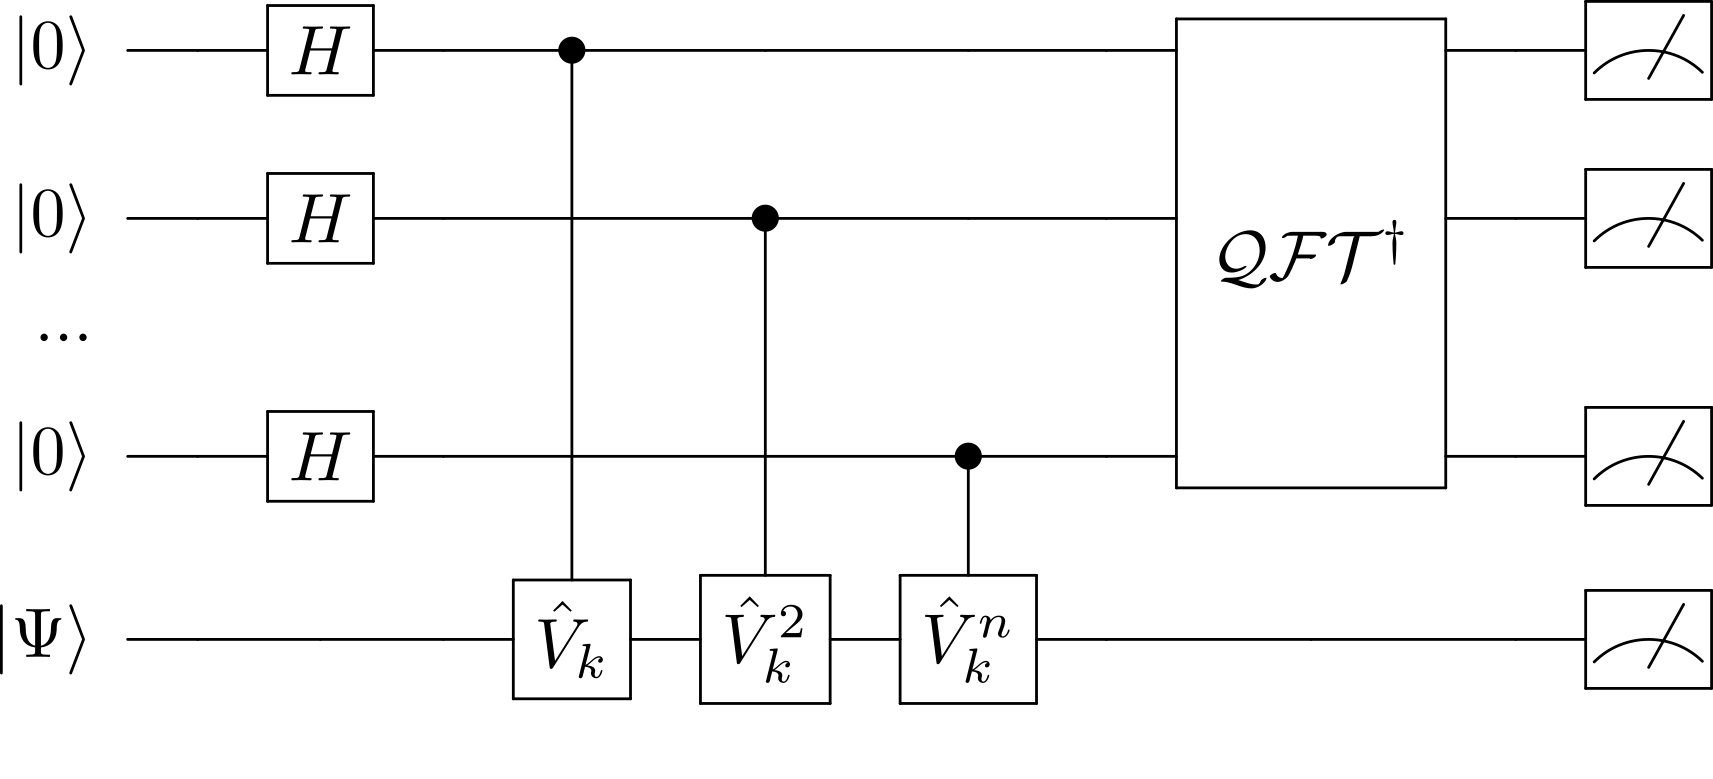
\includegraphics{/home/hrgrimsl/Lit/pea.png}
\end{center}
\end{figure}\\
In traditional phase estimation of a Hamiltonian, this circuit is run repeatedly with $\hat{V}_0$ defined in equation \ref{v0}. \cite{lloyd}
\begin{equation}\label{v0}
\hat{V}_0 = e^{-\frac{i}{\hbar}\hat{H}t}
\end{equation}
$\ket{\Psi}$ is an n-qubit reference state which is not orthogonal to the Hamiltonian eigenstates. \cite{lloyd}  A more detailed explanation of the algorithm is provided in appendix \ref{peaproof}, but the end result is a way to compute every eigenstate and eigenvalue of the Hamiltonian in polynomial time, provided the orthogonality requirement on the reference is met. \cite{lloyd}. Aspuru-Guzik and co. introduced a recursive variant of this scheme to require only a constant number of qubits in the readout register regardless of system size. \cite{alan} Unfortunately, the coherent evolution of $\ket{\Psi}$ required by PEA is beyond the reach of existing quantum hardware, motivating the development of the variational quantum eigensolver, or VQE. \cite{peruzzo} 
\end{paragraph}
\subsection{Variational Quantum Eigensolvers}
\begin{paragraph}{}
VQE fundamentally trades the coherence requirement of PEA for more measurements. \cite{peruzzo} In its original form (and the form of greatest interest to us,) Peruzzo and co. considered the UCC ansatz as a fixed unitary operator to replace the evolution unitary operator, limiting the parameter space to the dimension of the level of coupled cluster theory and guarenteeing polynomial scaling for any given level of truncation. \cite{peruzzo} In general, the Suzuki-Trotter approximation is employed to ameliorate computational expense of the UCC ansatz, and in some cases, improves the accuracy of the VQE. \cite{grimsley, joonho, suzuki} The approximation uses a truncated form of equation \ref{trotter}. \cite{suzuki}
\begin{equation}\label{trotter}
e^{A+B}=\lim_{n\to\infty}e^{A}e^{B}
\end{equation}
A rudimentary explanation of the necessity of the Trotter approximation is given in appendix \ref{trot}. The VQE algorithm variationally minimizes the expectation value of the parametrized ansatz, dividing the work between classical and quantum processors; the classical processor computes integrals, performs transforms, and runs a classical parameter optimization, outsourcing energy evaluations to the quantum processor. \cite{peruzzo}  While VQE is more feasible in the near future than PEA, methods which reduce coherence requirements even further are a subject of active investigation, leading to schemes like k-UPCCGSD and ADAPT. \cite{peruzzo,grimsley,joonho}
\end{paragraph}
\subsection{Toward NISQ Viability of VQE}
\begin{paragraph}{}
The endgame of quantum computing is to construct true, fault-tolerant quantum computers; however, this is unlikely to be feasible for many years. \cite{preskill} Of more interest is what Preskill dubbed the Noisy, Intermediate-Scale Quantum (NISQ) era, which anticipates the construction of 50-100 qubit quantum processors which cannot be manipulated, maintained, or measured with perfect fidelity. \cite{preskill} The NISQ regime is characterized by quantum processors becoming too large to simulate clasically; in the case of chemistry, this is expected to translate to running polynomial-time FCI calculations on larger systems than can be done with contemporary classical hardware. \cite{preskill, alan}  Algorithm design in this regime generally involves solving problems with as few quantum resources as possible, even if it means a dramatic increase in classical resource requirements; VQE is one such example of a "hybrid" method, but it has been (and is still being) improved in a variety of schemes since its inception. \cite{preskill, benedetti, grimsley, joonho}
\end{paragraph}
\begin{paragraph}{} 
Of particular promise are adaptive methods such as Adaptive Derivative-Assembled Pseudo-Trotterized (ADAPT) ansatz VQE. \cite{grimsley} While this type of scheme has been around less than a year, ADAPT has spawned interest in the physics community in developing similarly adaptive methods in other contexts, and continues to be a subject of research in our own group. \cite{benedetti,iqcc} The ADAPT algorithm is presented graphically in figure \ref{adapt}. \cite{grimsley}\begin{figure}[h!]\caption{ADAPT Algorithm}\label{adapt}

\includegraphics[width=\textwidth]{/home/hrgrimsl/posters/adapt-eps-converted-to.pdf}
\end{figure}  
\end{paragraph}
\begin{paragraph}{}
The algorithm begins with a reference state, generally the HF state.  At this point, we consider each of the operators in a predetermined pool. The HF state can be thought of as the HF state being acted on by one of the operators with the parameter $\theta=0$.  The energy gradient with respect to this operator is facile to compute, especially using the gradient algorithm derived by our group, and is not generally zero. \cite{grimsley} Every gradient is measured according to the formulas pictured in figure \ref{adapt}.  The operator giving the largest magnitude gradient is then permanently added to the ansatz.  The parameter $\theta$ is then optimized by gradient descent.  We repeat this process for the next gradient, reoptimizing all parameters with each addition to obtain a quasi-optimal ansatz.  Stopping criteria are presently somewhat arbitrary, and remain a subject of interest to our group.    
\end{paragraph}
\begin{paragraph}{}
The ADAPT ansatz is demonstrably more operator-compact than the large majority of possible random ans{\"a}tze for chemical systems, as shown in figure \ref{adaptplot}. \cite{grimsley} A key caveat to ADAPT's performance is that it is generally more parameter-efficient than its corresponding unitary coupled cluster method, even for strongly correlated systems such as $\mathrm{H_6}$. The ineffectiveness of untrotterized UCC is well-known in this regime, making it an area of great interest. \cite{evangelista}
\begin{figure}[h!]\caption{ADAPT Performances for Various Systems}\label{adaptplot}
plot
\end{figure}


\end{paragraph}


\section{Active Research}
\subsection{ADAPT Development}
\subsection{Demystifying Trotterization}
\subsection{Design of the ADAPT Operator Pool}



\appendix

\section{Jordan-Wigner Transformation}\label{jw}
\begin{paragraph}{}
We give here a brief overview of the Jordan-Wigner transfomation, the most intuitive mapping between fermionic and qubit operators.  Our second-quantized operators are tools for the spin-orbital basis, not for the $2^n$ occupation states of n qubits.  We seek then to define the annihilation operator $\sigma^-$ in the qubit basis, such that the anti-commutation relations pictured in \ref{anticomm} hold. \cite{szabo} 
\begin{align}\label{anticomm}
 \{\sigma^+_j,\sigma_k^-\}&=\delta_{jk}\\
 \{\sigma^-_j,\sigma_k^-\}&=0\nonumber
\end{align}
where $\sigma^+=\left(\sigma^{-}\right)^\dagger}$.
Consider the action of the annihilation operator on an occupation product state $\ket{\alpha}=\otimes_{i=1}^n\ket{\alpha_i}$ given in \ref{deriv1}, where each $\alpha_i$ is restricted to 0 or 1, and $\sigma_j$ has the same properties as the fermionic annihilation operator such that it maps $\ket{1}$ to $\ket{0}$ and $\ket{0}$ to 0. \cite{jwnotes} 
\begin{align}\label{deriv1}
\sigma^{-}_j\ket{\alpha} &= \sigma^{-}_j\ket{\alpha_1}\otimes_{i=2}^n\ket{\alpha_i}\\ 
\nonumber&=\sigma^{-}_j \left(\sigma^{\dagger}_1\right)^{\alpha_1}\otimes_{i=2}^n\ket{\alpha_i}\\
\nonumber&=-1^{\alpha_1}\ket{\alpha_1}\sigma^{-}_j\otimes_{i=2}^n\ket{\alpha_i}\\
\nonumber&=Z\ket{\alpha_1}\sigma^{-(2)}_j\otimes_{i=2}^n\ket{\alpha_i}\\
\nonumber&\text{Repeat j-2 additional times}\\
\nonumber&=\otimes_1^{i=j-1}Z\ket{\alpha_i}\sigma^{-(j)}_j\ket{\alpha_j}\otimes_{i=j+1}^n\ket{\alpha_i}\\
\nonumber&=\otimes_1^{i=j-1}Z\ket{\alpha_i}\ket{0}\braket{1|\alpha_j}\otimes_{i=j+1}^n\ket{\alpha_i}
\end{align}
where $\sigma^{-(j)}$ acts only on qubits of index j or greater.  Similarly, the creation operator acting on $\ket{\alpha}$ produces \ref{dag.}
\begin{equation}\label{dag}
\nonumber&\otimes_1^{i=j-1}Z\ket{\alpha_i}\ket{1}\braket{0|\alpha_j}\otimes_{i=j+1}^n\ket{\alpha_i}
\end{equation}
It follows from the definitions of the Pauli operators that: 
\begin{equation}\label{sigmat}
\sigma_j^- = -\frac{1}{2}Z\otimes_1^{j-1}(X-iY)I\otimes_{j+1}^n\\
\sigma_j^+ = -\frac{1}{2}Z\otimes_1^{j-1}(X+iY)I\otimes_{j+1}^n\\
\end{equation}
It can be shown that both of the anti-commutation relations in \ref{anticomm} hold for these operators.  Consequently, the Jordan-Wigner transformation allows the Pauli string expression of any operator or vector which we know how to express in terms of creation and annihilation operators.  This includes initial states, Hamiltonians, and parametrized excitations.  Naturally, this extends to the unitary coupled cluster ansatz.
\end{paragraph}
\section{Suzuki-Trotter Decomposition Background}\label{trot}
\begin{paragraph}{}
The Suzuki-Trotter decomposition is generally considered in the context of time evolution operators such as the propagator $e^{i\hat{H}}$; using a finite product of these ``slices" is equivalent to using finite time steps to approximate the evolution. \cite{hastings, babbush, suzuki} It follows that in the limit of infinite slices, one obtains the true evolution. \cite{suzuki} However, finite truncations of the Trotter decomposition suffer not only from truncation error, but are not generally uniquely defined; in general, there is no reason to expect the unitary operators used to commute, and Trotter error is well-understood as a source of error in evaluating the Hamiltonian. \cite{hastings}  The effect of unitary coupled cluster ansatz decomposition ordering remains unexplored in the literature, and has become an active area of research for our group.  In \ref{trotsky}, we give examples of untrotterized, first-order trotterized, and second-order trotterized ans{\"a}tze.
\begin{align}\label{trotsky}
\text{{Untrotterized:}}&\hspace{40pt}&e^{A\theta_a+B\theta_b+...}&=e^{B\theta_b+A\theta_a+...}\\
\text{{First-order trotterized:}}&&e^{A\theta_a}e^{B\theta_b}...&\neq e^{B\theta_b}e^{A\theta_a}...\nonumber\\
\text{{Second-order trotterized:}}&&\left(e^{\frac{A\theta_a}{2}}e^{\frac{B\theta_b}{2}}...\right)^2&\neq \left(e^{\frac{B\theta_b}{2}}e^{\frac{A\theta_a}{2}}...\right)^2\nonumber
\end{align}
Note the lack of uniqueness in all finite Trotter decompositions.
\end{paragraph}


\section{Phase Estimation Algorithm Details}\label{peaproof}
Here we provide more detailed explanations of the phase estimation algorithm and the recursive variant developed by Aspuru-Guzik and co.\cite{lloyd, alan} Referring to figure \ref{pea} will be helpful for the latter.
\subsection{Traditional Phase Estimation \cite{lloyd}}
\begin{paragraph}{}
This scheme begins by using the n-qubit Hadamard gate to obtain a linear combination of each of the states which can be obtained in an n-qubit working register according to equation\ref{hn}.
\begin{align}\label{hn}
H^{\otimes n}\ket{0}^{\otimes n}\ket{\Psi}=\frac{1}{\sqrt{N}}\sum_{i}\ket{i}\ket{\Psi}
\end{align}
An input register is initialized to some arbitrary phase $\ket{\Psi}$ which (hopefully) has non-zero overlap with the true eigenvectors of the system.  At this point, a series of controlled unitary gates $\hat{V}^i$ is prepared; the specific gates of this preparation depend on hardware capabilities.  This leads eventually to the preparation of the state in \ref{ft}, using the spectral decomposition of $\ket{\Psi}$ with respect to $\hat{V}$.
\begin{align}\label{ft}
\frac{1}{\sqrt{N}}\sum_i \ket{i}\hat{V}^i\ket{\Psi}\equiv \frac{1}{\sqrt{N}}\sum_{i\lambda}\ket{i}\hat{V}^ic_\lambda \ket{\lambda}
\end{align}
Taking $\lambda$ to be the eigenvalue associated with $\ket{\lambda}$, this becomes represented by \ref{spec}.
\begin{align}\label{spec}
\frac{1}{\sqrt{N}}\sum_{i\lambda}c_\lambda\lambda^i\ket{i}\ket{\lambda}
\end{align}
Defining $\lambda$ by equation \ref{phase}, using $\hat{j}$ as the imaginary unit, we can perform a quantum Fourier transform to obtain the phase $\omega_\lambda$ and consquently the $\lambda$ for whatever we measure the system in.  Repeated evaluations allow the determination of all eigenstates and eigenvalues, obtaining accuracy which is theoretically identical to FCI.
\begin{align}\label{phase}
\lambda =  e^{i\omega_\lambda \hat{j}}
\end{align}
\end{paragraph}
\subsection{Recursive Phase Estimation \cite{alan}}
\begin{paragraph}{}
The primary advantage of this algorithm is the ability to obtain high precision with a small number of working qubits.  The recursive algorithm begins with a four-qubit PEA regardless of system size; giving the phase of the ground state $\omega$ (and consequently $\lambda_0$) with a precision of 1/16.  The time evolution operator $\hat{V}_0$ is replaced now with \ref{iter}, and another PEA is conducted.  Squaring $\hat{V}_0$ and dividing out the approximate ground state energy causes a phase shift and ensures that the second PEA will only search the space of improvements on this eigenstate, giving approximate precision .004.  This is repeated to an arbitrary degree of precision.
\begin{equation}\label{iter}
\hat{V_1}={\frac{1}{\lambda_0}\hat{V_0}}^2
\end{equation}
\end{paragraph}

\section{Efficient Classical Gradient Computation}\label{gradientalgorithm}
\begin{paragraph}{}
While analytic formulae for the gradient of the trotterized UCC ansatz have existed for a few years now, in ref. \citenum{grimsley} we derived the most tractable algorithm by far for this evaluation on a classical computer. \cite{crooks, grimsley, romero, guerreschi}  We outline here the proof and execution details of this recursive algorithm. We begin by expanding the analytic derivative and recognizing some basic identities in \ref{gradient}.
\begin{align}\label{gradient}
\frac{\partial E}{\partial \theta_k}&=\frac{\partial}{\partial\theta_k}\bra{HF}e^{-A\theta_a}...e^{-K\theta_k}...e^{-Z\theta_z}\hat{H}e^{Z\theta_z}...e^{K\theta_k}...e^{A\theta_a}\ket{HF}\\
&=\bra{HF}...e^{-K\theta_k}...\hat{H}...Ke^{K\theta_k}...\ket{HF}-\bra{HF}...Ke^{-K\theta_k}...\hat{H}...e^{K\theta_k}...\ket{HF}\nonumber\\
\nonumber&=2\mathcal{R}\bra{HF}...e^{-K\theta_k}...\hat{H}...Ke^{K\theta_k}\ket{HF}
\end{align}
Because we intend to evaluate a large number of gradients, we introduce a recursive scheme to obtain all of the gradients between A and Z.  We define some useful quantities in \ref{defs}.
\begin{align}\label{defs}
\bra{\psi^H_{\{A,...,N\}}}&=\bra{HF}e^{-A\theta_a}...e^{-Z\theta_z}\hat{H}e^{A\theta_a}...e^{N\theta_n}\\\nonumber \ket{\psi_{\{A,...,N\}}}&=e^{N\theta_n}...e^{A\theta_a}\ket{HF}
\end{align}
We recognize that
\begin{equation}\label{init}
\frac{\partial E}{\partial \theta_a}=  2\mathcal{R}\bra{\psi^H_\emptyset}A\ket{\psi^H_{\{A,...,Z\}}}
\end{equation}
Computing \ref{init} requires evaluating N exponential matrix actions, where N is the number of unitary operators in the ansatz.  (It is not 2N, because both terms in \ref{init} are related by transposition and multiplication by the Hamiltonian.)  Additionally
\begin{equation}\label{recurse1}
\frac{\partial E}{\partial \theta_b}=\bra{\psi^H_{\{A\}}}B\ket{\psi_{\{B,...Z\}}}
\end{equation}
Computing \ref{recurse1} only requires two exponential matrix actions, because
\begin{align}\label{recurse2}
\bra{\psi^H_{\{A\}}} & = \bra{\psi^H_\emptyset} e^{A\theta_a}\\
\ket{\psi_{\{B,...Z\}}} & = e^{-A\theta_a}\ket{\psi_{\{A,...,Z\}}}
\end{align}  
This procedure can be repeated N times for a total of 3N exponentiated matrices to compute the complete gradient.
\end{paragraph}
\bibliography{References/References.bib}

\end{document}
